
\chapter{Algoritmo BRKGA con búsqueda local para TOP}

En el presente capítulo describiremos en detalle la solución implementada para el \textit{Team Orienteering Problem}. La implementación se la puede dividir en 3 módulos importantes. Primero el decodificador, que como mencionamos en el capítulo BRKGA tiene la tarea de convertir un arreglo de enteros aleatorios en una solución válida del problema. Luego el algoritmo BRKGA, cuya implementación puede hacerse con total independencia del problema a resolver. Por último las búsquedas locales aplicadas en cada nueva generación a los mejores individuo de la población. 

\bigskip

TODO: Agregar mencion de resultados de BDM

En el capítulo \textit{Resultados} se mostrará en detalle los resultados obtenidos de la versión final de la implementación sobre el benchmark de problemas de Chao y Tsiligirides \cite{IntancesChaoTsiligirides}. Se compararon los resultados con los obtenidos de los trabajos previos de Chao et al. \cite{ChaoGoldenWasil} (CGW), de Archetti et al. \cite{ArchettiHertzSperanza} (AHS) y los de Tang and E. Miller-Hooks \cite{TangMillerHooks} (TMH).

\bigskip

En este capítulo mostré los resultados parciales obtenidos a lo largo del desarrollo de la implementación. A modo de analizar el rendimiento de una solución de forma simple y rápida cree un índice que llamo \textit{índice de efectividad} ($i_e$). El $i_e$ muestra que tan buena es la solución encontrada. Esto se hace comparando el beneficio de mi solución encontrada con el beneficio de la mejor solución para el la misma instancia del problema. Se utilizaron los resultados de los trabajos previos mencionados para crear el índice de efectividad. Es importante destacar que el $i_e$ no es la función objetivo. La función objetivo es maximizar el beneficio a recolectar. 

\bigskip

Se seleccionó un subconjunto del benchmark de instancias de problemas de Chao y Tsiligirides \cite{IntancesChaoTsiligirides} para medir el progreso de mi desarrollo. Las seis instancias seleccionadas varían en cantidad de clientes y vehículos, esto es importante para que el análisis del rendimiento sea lo más objetivo posible. Luego de obtener una solución para cada una de estas instancias, se calcula el $i_e$ que definí de la siguiente manera:

TODO: Agregar profit de resultados de BDM

\begin{equation}
bestProfit(i) = max(profit(CGW(i)), profit(AHS(i)), profit(TMH(i))) \label{eq:bestProfit}
\end{equation}
\begin{equation}
i_e(imp_{v.xyz},i) = profit(imp_{v.xyz}(i)) / bestProfit(i) \label{eq:efectividad}
\end{equation}

\bigskip

De la primera ecuación \eqref{eq:bestProfit} obtenemos el mejor beneficio de entre los trabajos previos seleccionados para la instancia $i$. Luego en la función \eqref{eq:efectividad} calculo que tan efectiva es la versión $xyz$ de mi implementación para la instancia $i$. Esto se hace dividiendo el beneficio obtenido de mi implementación sobre el mejor beneficio calculado previamente. Luego analizar el rendimiento de $i_e$ es muy sencillo. Si $i_e = 1$, la solución encontrada es tan buena como la mejor solución encontrada hasta el momento. Si $0.90 < i_e < 1$, luego la solución encontrada no es tan buena como la mejor pero la considero competitiva.

\bigskip

Se explicará en detalle el funcionamiento de los módulos que componen la implementación, incluyendo su pseudocódigo y los resultados parciales obtenidos luego de implementar tal módulo. El pseudocódigo utilizado sigue la sintaxis de c\#, el lenguaje en el cual implemente el desarrollo. El objetivo del pseudocódigo es ilustrar el comportamiento del método que representa, tal método es implementado con ciertas variaciones que no viene al caso describir. Considere que no aportaba a su descripción las lineas de código relacionadas con: medición de tiempo, monitoreo de estados, testing, manejo de excepciones, persistencia de resultados, etc. 


\bigskip

Para la valuación de $i_e$ se eligieron seis instancias del benchmark \cite{IntancesChaoTsiligirides} de modo que fueran variadas entre sí. Tome dos pequeñas, dos medianas y dos grandes, cuyas descripción pueden observarse en la siguiente tabla:

\begin{center}
\begin{tabular}{ |c|c|c|c|c| } 
 \hline
Autor & Instancia & Nodos & Vehículos & tMax \\
\hline
Tsiligirides & p2.2.k & 21 & 2 & 22.50 \\
Tsiligirides & p2.3.g & 21 & 3 & 10.70 \\
Tsiligirides & p3.4.p & 33 & 4 & 22.50 \\
Chao & p5.3.x & 66 & 3 & 40.00 \\
Chao & p7.2.e & 102 & 2 & 50.00 \\
Chao & p7.4.t & 102 & 4 & 100.00 \\
 \hline
\end{tabular}
\end{center}


\bigskip

Las tablas donde mostraré el $i_e$ y el beneficio de los resultados parciales tendrá un subconjunto de los siguientes encabezados:

\begin{center}
\begin{tabular}{ |c|c|c|c|c|c|c|c|c|c|c|c|c| } 
 \hline
$I$ & $\#N$ & $\#V$ & $tMax$ & $C$ & $\#S$ & $T_{avg}$ & $B_{max}$ & $B_{min}$ & $B_{avg}$ & $i_{eMax}$ & $i_{eAvg}$ & $BTP_{max}$ \\
\hline
\end{tabular}
\end{center}

\bigskip

Descripciones:
\begin{itemize}
	\item \textbf{$I$}: Nombre de la instancia.
	\item \textbf{$\#N$}: Cantidad de nodos (clientes mas punto de partida y fin de recorrido) de la instancia.
	\item \textbf{$\#V$}: Cantidad de vehículos de la instancia.
	\item \textbf{$tMax$}: Distancia máxima de la ruta de cada vehículos de la instancia.
	\item \textbf{$C$}: Configuración general del BRKGA. Es un código que sintetiza la configuración básica global, explicado en detalle más adelante (ver sección \label{sec:descrCongif}).
	\item \textbf{$\#S$}: Cantidad de soluciones de las cuales se sacaron los datos.
	\item \textbf{$T_{avg}$}: Tiempo promedio en milisegundos de la ejecución total de la implementación.
	\item \textbf{$B_{max}$}: Beneficio máximo de las \#S soluciones generadas.
	\item \textbf{$B_{min}$}: Beneficio mínimo de las \#S soluciones generadas.
	\item \textbf{$B_{avg}$}: Beneficio promedio de las \#S soluciones generadas.
	\item \textbf{$i_{eMax}$}: Indice de efectividad máximo. Utilizado en los resultados finales. Utilizo mi mejor beneficio obtenido para una instancia \eqref{eq:efectividad}.
	\item \textbf{$i_{eAvg}$}: Indice de efectividad promedio. Utilizado en los resultados parciales. Utilizo el promedio de los beneficios obtenidos para una misma instancia \eqref{eq:efectividad}.
	\item \textbf{$BTP_{max}$}: Beneficio de Trabajos Previos máximo para la misma instancia. Los trabajos previos son: CGW \cite{ChaoGoldenWasil}, AHS \cite{ArchettiHertzSperanza} y TMH \cite{TangMillerHooks}.
\end{itemize}

TODO: Agregar mención de resultados de BDM arriba

\section{Decodificador}

El decodificador debe generar una solución valida del problema dado un vector aleatorio de enteros y conociendo la instancia del problema (vehículos disponibles, clientes, tmax, etc). Con tal objetivo construye una solución valida asignando clientes a las rutas de los vehículos disponibles respetando \textit{tMax}, su distancia máxima de recorrido. El orden en que toma los clientes a asignar es clave y determina la solución resultante. Es el vector de enteros aleatorios quien determina el orden en el cual se tomarán los clientes para asignarlos a una ruta. Por lo tanto el vector tendrá una longitud equivalente a la cantidad de clientes del problema (nodos con beneficio mayor a cero).

\bigskip

Propuse dos decodificadores, uno al cual llamo \textit{Decodificador Simple} y otro que llamé \textit{Decodificador Goloso}. Ambos decodificadores tienen sus ventajas y desventajas.

\subsection{Orden de los clientes a considerar}\label{sec:ordenDeco}

Dado una instancia de un problema con $n$ clientes y un vector de enteros aleatorio de tamaño $n$, un decodificador genera una solución valida de un problema. El vector, en mi implementación, es un vector de \textit{RandomKeys}. Un \textit{RandomKey} tiene dos propiedades, el entero aleatorio llamado \textit{Key} y otro entero llamado \textit{ClientId} como podemos ver en a continuación. 

\bigskip

\begin{lstlisting} 
public class RandomKey
{        
	public int Key { get; private set; }
	public int ClientId { get; private set; }
}
\end{lstlisting}

\bigskip

El propósito de $ClientId$ es mapear un \textit{RandomKey} con un \textit{Cliente}. Existe un vector de \textit{Clientes} en el Mapa del problema, a cada \textit{Cliente} se le asigna un identificador que es un numero entero en el intervalo $[1, \#Clientes]$. Luego para un vector de \textit{RandomKeys} de tamaño $\#Clientes$ no existen dos \textit{RandomKeys} con mismo valor de \textit{ClientId} y todos los \textit{ClientId} se encuentran en el intervalo $[1, \#Clientes]$. De esta forma cada \textit{RandomKey} siempre mapea con un solo \textit{Cliente}. Luego de mapear cada \textit{Cliente} con su correspondiente \textit{RandomKey}, se los ordena de forma ascendente por el \textit{Key} del \textit{RandomKey} con el cual mapeo. Este es el orden por el cual se tomaran los clientes para ser asignados a los vehículos. Podemos ver esto sintetizado en una linea de pseudocódigo en \ref{lst:GetOrderedClients}. La figura \ref{fig:RandomKeysOrdenando} muestra como ordenamos un vector de \textit{RandomKeys}.

\bigskip

\begin{lstlisting} [label={lst:GetOrderedClients}]
public List<Client> GetOrderedClients(List<RandomKey> randomKeys)
{        
	return randomKeys.OrderBy(r => r.Key).Select(r => Map.Clients[r.ClientId]);
}
\end{lstlisting}

\begin{figure}[h]
	\caption{RandomKeys ordenando clientes}
	\centering
	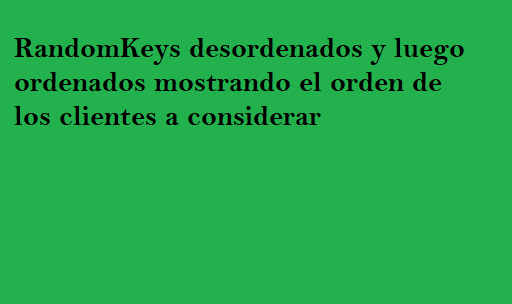
\includegraphics[width=14cm]{RandomKeysOrdenando}
	\label{fig:RandomKeysOrdenando}
\end{figure}

\subsection{Decodificador simple}

El decodificador simple recibe como parámetro el vector de enteros aleatorios y lo primero que hace es obtener los clientes ordenados como describimos anteriormente. Luego por cada vehículo, si el siguiente cliente se puede incluir en la ruta se incluye sino considera que la ruta esta completa y pasa al siguiente vehículo. Estos se puede ver en detalle en el pseudocódigo \ref{lst:Decode}. 

\bigskip

\begin{lstlisting} [label={lst:Decode}]
public Solution Decode(List<RandomKey> randomKeys, ProblemInfo pi)
{
	var clients = GetOrderedClients(randomKeys);
	var vehicles = pi.GetVehicles();	
	var iv = 0;
	var ic = 0;	
	do
	{
		if(vehicles[iv].CanVisit(clients[ic]))
		{
			vehicles[iv].AddClient(clients[ic]);
			ic++;
		}
		else
		{
			iv++;			
		}
		
	} while(iv < vehicles.Length && ic < clients.Length)	
	var solution = pi.InstanceSolution(vehicles);
	return problem;
}
\end{lstlisting}

Un cliente $c_i$ se puede agregar a la ruta si al agregarlo, la ruta no supera su distancia máxima permitida. Sean $v$ vehículo, $tMax$ la distancia máxima de $v$, $tAct$ la distancia actual de $v$, $f$ el destino final de la ruta, $c_u$ el ultimo cliente agregado a la ruta de $v$ y $c_i$ cliente a evaluar agregar a la ruta de $v$. Como podemos observar en el pseudocódigo \ref{lst:Decode}, cree un método llamado \textit{CanVisit} que retorna \textit{true} cuando $c_i$ se puede agregar a la ruta y \textit{false} en caso contrario. El método \textit{CanVisit} modela la siguiente fórmula:

\bigskip

\( tAct\, +\, distancia(c_u, c_i)\, +\, distancia(c_i, f)\, -\, distancia(c_u, f) \leq tMax\)

\bigskip

Una vez que termine de implementar el decodificador simple, analice el rendimiento de las soluciones generadas a partir de este decodificador. Hice este análisis para saber que tan buena sería la población inicial de mi algoritmo BRKGA si utiliza el decodificador simple. Para realizar el análisis cree 200 vectores $RandomKeys$ que el decodificador simple convirtió en 200 soluciones validas del problema. Luego se calculó el beneficio máximo, promedio, mínimo y el índice de efectividad promedio. Esto se repitió para las seis instancias del benchmark seleccionadas anteriormente. La siguiente tabla tiene los resultados obtenidos:

\begin{center}
\begin{tabular}{ |c|c|c|c|c|c|c|c|c|c| } 
\hline
$I$ & $\#N$ & $\#V$ & $tMax$ & $\#S$ & $B_{max}$ & $B_{min}$ & $B_{avg}$ & $i_{eAvg}$ & $BTP_{max}$ \\
\hline
p2.2.k & 21 & 2 & 22.50 & 200 & 175 & 40 & 102 & 0.37 & 275  \\
p2.3.g & 21 & 3 & 10.70 & 200 & 140 & 45 & 83 & 0.57 & 145  \\
p3.4.p & 33 & 4 & 22.50 & 200 & 270 & 90 & 170 & 0.30 & 560  \\
p5.3.x & 66 & 3 & 40.00 & 200 & 405 & 195 & 295 & 0.19 & 1555  \\
p7.2.e & 102 & 2 & 50.00 & 200 & 98 & 8 & 39 & 0.13 & 290  \\
p7.4.t & 102 & 4 & 100.00 & 200 & 221 & 40 & 116 & 0.11 & 1077  \\
\hline
\end{tabular}
\end{center}

En estos resultados podemos observar que para instancias pequeñas los resultados son mejores. Notar como $i_{eAvg}$ disminuye a medida que la instancia tiene mayor numero de clientes ($\#N$).

\subsection{Características y debilidades del decodificador simple}

Este decodificador es simple y rápido, su orden de complejidad es de $O(\#clientes + \#vehiculos)$. En la practica nunca se llega recorrer todos los clientes ya que cambia de vehículo en cuanto encontró un cliente que no logro insertar en su ruta. Por lo tanto en la practica nunca llega al orden de complejidad mencionado. Esto es una gran ventaja ya que en cada iteración del BRKGA se va a decodificar una cantidad $\#Poblacion$ de veces. Luego una decodificación rápida nos permitirá mayor cantidad de generaciones.

\bigskip

Una característica menos relevante es el orden en que quedan los clientes asignados en los vehículos al ver el vector de \textit{RandomKeys}.  Sea $v$ el vector de clientes ordenados por un vector aleatorio de enteros. Existen $m+1$ indices $i_0 = 0, i_1, i_2, .., i_m$ donde $m$ es la cantidad de vehículos y $0 \leq i_j \leq \#clientes$ tales que el vehículo $j$ incluye en su recorrido a todos los clientes del subvector $v[i_{j-1}, i_j-1]$. Luego todos los clientes en el subvector $v[i_m, v.Length - 1]$ son clientes no alcanzados por la solución. En otras palabras, los clientes quedan agrupados por vehículo cuando los vemos en el vector ordenado. Esto puede verse en la figura \ref{fig:DistribucionClientesDecoSimple}.

\begin{figure}[h]
	\caption{Posible distribución de clientes utilizando el decodificador simple para el vector de RandomKeys de ejemplo. La primer ruta visita primero al cliente 6 y luego al 2. Como no pudo incluir al cliente 5, se cerró la ruta del primer vehículo y siguió con el próximo vehículo disponible. La segunda ruta visita al cliente 5 y luego al cliente 1. Como no pudo visitar al cliente 4 por la limitación de tiempo, no intento agregar a los siguientes clientes.}
	\centering
	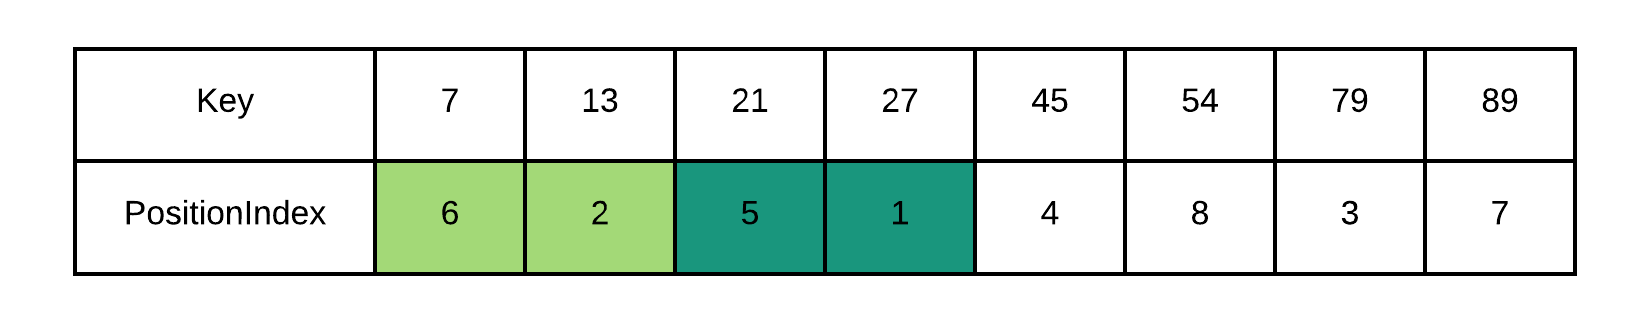
\includegraphics[width=14cm]{DistribucionClientesDecoSimple}
	\label{fig:DistribucionClientesDecoSimple}
\end{figure}

\bigskip

Un problema que tiene este decodificar es en la existencia de un cliente inalcanzable, es decir si existe $c$ cliente tal que:

\bigskip

\( distancia(i, c)\, +\, distancia(c, f)\, >\, tMax\)

\bigskip

Esto puede generar soluciones de la población donde existan vehículos con rutas vacías. Supongamos que existe un cliente inalcanzable y que es el primer cliente en ser considerado a agregar a la ruta de un vehículo, como el cliente es inalcanzable no entra en la ruta del primer vehículo luego se considera que el vehículo tiene la ruta completa y se pasa con el siguiente vehículo y así sucesivamente. La solución fácil a este problema es filtrando todos los clientes inalcanzables previo a la ejecución del BRKGA. Esta solución es la mejor y mas barata ya que reducimos el tamaño del problema antes de comenzar a resolverlo.

\bigskip

Otro problema que tiene este decodificador es que cambia de vehículo al primer intento fallido de expandir su ruta. Luego puede generar soluciones con rutas muy pequeñas, por este motivo implementé el \textit{Decodificador Goloso}.


\subsection{Decodificador Goloso}

El decodificador goloso en principio funciona igual que el decodificador simple hasta que llega a un cliente que no pudo agregar a la ruta de un vehículo. En este caso, en vez de pasar a trabajar con el siguiente vehículo disponible, intenta agregar al siguiente cliente y así sucesivamente hasta que no hay mas clientes que intentar. Luego al pasar al siguiente vehículo intenta solamente con los clientes no asignados a los vehículos anteriores y siempre respetando el orden de los clientes asignado por el vector de enteros aleatorios.

\bigskip

\begin{lstlisting} 
public Solution Decode(List<RandomKey> randomKeys, ProblemInfo pi)
{
	var clients = GetOrderedClients(randomKeys);
	var cIterator = new Iterator(clients);
	var vehicles = pi.GetVehicles();	
	var iv = 0;
	while(iv < vehicles.Length)
	{
		var currentClient = cIterator.Next;
		while(currentClient != null)
		{
			if(vehicles[iv].CanVisit(currentClient))
			{
				vehicles[iv].AddClient(currentClient);
				cIterator.Remove(currentClient);
			}
			currentClient = cIterator.Next;
		}
		cIterator.ToStartingPosition;
	}
	var solution = pi.InstanceSolution(vehicles);
	return problem;
}
\end{lstlisting}

\bigskip

Con esta modificación su orden complejidad aumenta a $0(\#clientes * \#vehiculos)$. El metodo \textit{decode} es usado tantas veces que este a lo largo del BRKGA que este pequeño aumento en su complejidad algorítmica tiene un impacto visible en el tiempo de ejecución. Por otro lado, en promedio aumenta el beneficio de las soluciones generadas por el decodificador. Esa es la compensación que tenemos entre el decodificador simple y el goloso. 

\bigskip

Una observación de menor importancia que podemos hacer sobre el decodificador goloso es que al observar el vector ordenado de \textit{RandomKeys}, ya no tenemos los clientes de forma continua según su vehículo asignado como sucedía con el decodificador simple. Esto puede verse en la figura \ref{fig:DistribucionClientesDecoGoloso}.

\begin{figure}[h]
	\caption{Posible distribución de clientes utilizando el decodificador goloso para el vector de RandomKeys de ejemplo. La primer ruta visita a los clientes 6, 2 y por último al 8. El decodificador goloso no cerró la ruta del primer vehículo al no poder incluir el cliente 5, intenta en orden con el resto de los clientes aún no visitados y logra insertar el cliente 8. De un modo simlilar, sucede con la segunda ruta al no poder incluir al cliente 4.}
	\centering
	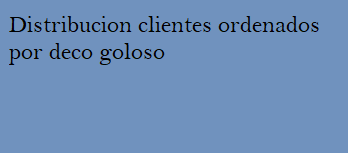
\includegraphics[width=14cm]{DistribucionClientesDecoGoloso}
	\label{fig:DistribucionClientesDecoGoloso}
\end{figure}

\bigskip

Del mismo modo que hice con el decodificador simple, le hice el mismo análisis de rendimiento al decodificador goloso. Genere otros 200 vectores de \textit{RandomKeys} para cada una de las mismas seis instancias de problemas y el decodificador goloso creo 200 soluciones validas para cada uno de seis los problemas:

\begin{center}
\begin{tabular}{ |c|c|c|c|c|c|c|c|c|c| } 
\hline
$I$ & $\#N$ & $\#V$ & $tMax$ & $\#S$ & $B_{max}$ & $B_{min}$ & $B_{avg}$ & $i_{eAvg}$ & $BTP_{max}$ \\
\hline
p2.2.k & 21 & 2 & 22.50 & 200 & 260 & 95 & 164 & 0.60 & 275   \\
p2.3.g & 21 & 3 & 10.70 & 200 & 140 & 95 & 122 & 0.84 & 145   \\
p3.4.p & 33 & 4 & 22.50 & 200 & 410 & 180 & 288 & 0.51 & 560   \\
p5.3.x & 66 & 3 & 40.00 & 200 & 525 & 305 & 412 & 0.26 & 1555   \\
p7.2.e & 102 & 2 & 50.00 & 200 & 163 & 31 & 96 & 0.33 & 290   \\
p7.4.t & 102 & 4 & 100.00 & 200 & 438 & 160 & 280 & 0.26 & 1077   \\
\hline
\end{tabular}
\end{center}

Todos los resultados promedio, mínimo y máximos mejoran considerablemente. Tal es así, que el $i_{eAvg}$ en algunos casos es mayor al doble de lo obtenido con en el decodificador simple. Por otro lado, se vuelve a observar como disminuye $i_{eAvg}$ a medida que crece el tamaño de la instancia del problema.

\section{Biased Random Key Genetic Algorithms}

En una primera instancia se implementa un BRKGA estándar. Dado una instancia de un problema, primero se genera la población inicial. Luego mientras no se cumpla la condición de parada, evolucionamos la población. Es decir creamos una nueva generación de soluciones a partir de la generación anterior como se explicó en la sección BRKGA ~(ver sección~\ref{sec:brkga}).

\bigskip

A continuación muestro el pseudocódigo de una vista macro general del algoritmo BRKGA implementado:

\bigskip

\begin{minipage}{\textwidth}
\begin{lstlisting} 
public Solution RunBrkga(ProblemManager problemManager)
{
    ProblemManager.InitializePopulation();

    while (!ProblemManager.StoppingRuleFulfilled())
        ProblemManager.EvolvePopulation();

    return ProblemManager.Population.GetMostProfitableSolution();
}
\end{lstlisting}
\end{minipage}

\bigskip

El objeto \textit{ProblemManager} es el orquestrador del BRKGA, se setea con un objeto \textit{Configuración} y el objeto \textit{PopulationGenerator}. Tiene acceso de forma indirecta, a través de \textit{PopulationGenerator}, de toda la información del problema (vehículos, clientes, tMax, etc.).

\subsection{Configuración}

A modo de poder testear distintas configuraciones del BRKGA, se creo un objeto \textit{Configuration} que setea todas las configuraciones que impactan en el resultado final del BRKGA. Este objeto es esencial para tunear el implementación de una forma rápida y ordenada. Al centralizar todas las variables que podrían impactar en resultado final, ganaba mucho tiempo al testear variaciones de mi implementación. Además, al estar centralizada toda la información variable se obtiene una lectura veloz del BRKGA que se está usando. En otras palabras incrementamos nuestra capacidad de monitoreo y control del desarrollo. A continuación el objeto \textit{Configuration} y sus propiedades:

\bigskip

\begin{minipage}{\textwidth}
\begin{lstlisting}
public class BrkgaConfiguration
{
	public string Description { get; }
	public int MinIterations { get; set; }
	public int MinNoChanges { get; set; }
	public int PopulationSize { get; set; }
	public decimal ElitePercentage { get; set; }
	public decimal MutantPercentage { get; set; }
	public int EliteGenChance { get; set; }
	public List<ILocalSearchHeuristic> Heuristics { get; set; }
	public int ApplyHeuristicsToTop { get; set; }
	public DecoderEnum DecoderType { get; set; }
	
	private void SetDescription();
}
\end{lstlisting}
\end{minipage}

\bigskip

\subsection{Descripción y codificación de las propiedades del objeto configuración}\label{sec:descrCongif}
Descripción de las propiedades del objeto Configuración:

\begin{itemize}
  \item \textbf{Description}: Es una especie de hash descriptivo de la instancia del objeto. Su funcionalidad es poder identificar rápidamente la configuración global del BRKGA. Solo puede ser seteado con el metodo SetDescription() que utiliza la clave y el valor de el resto de las propiedades.
  \item \textbf{MinIterations}: Clave \textbf{MI}. Valor entero utilizado en la función de corte. Cantidad mínima de generaciones que debe completar el BRKGA para finalizar. 
  \item \textbf{MinNoChanges}: Clave \textbf{MNC}. Valor entero utilizado en la función de corte. Cantidad de generaciones sin modificaciones del mejor beneficio necesario para cortar el algoritmo BRKGA.
  \item \textbf{PopulationSize}: Clave \textbf{PS}. Valor entero denota el tamaño de la población.
  \item \textbf{ElitePercentage}: Clave \textbf{EP}. Valor decimal en el intervalo $(0, 1)$ que determina el tamaño de la población elite. 
  \item \textbf{MutantPercentage}: Clave \textbf{MP}. Valor decimal en el intervalo $(0, 1)$ que determina el tamaño mínimo de la población mutante. 
  \item \textbf{EliteGenChance}: Clave \textbf{EGC}. Valor entero en el intervalo $(0, 100)$ que determina la probabilidad que tiene el alelo del padre elite, en transmitirse a su descendiente. 
  \item \textbf{Heuristics}: Clave \textbf{HEU}. Secuencia de algoritmos de búsquedas locales que se le aplicaran a la mejor solución de cada generación, a la cual no se le hayan aplicado las búsquedas locales aún. Se implementaron cuatro búsquedas locales (Su desarrollo sera explicado mas adelante en otra sección.):
	\begin{itemize}
		\item \textbf{Swap}: Valor \textbf{S}.
		\item \textbf{Insert}: Valor \textbf{I}.
		\item \textbf{2-Opt}: Valor \textbf{O}.
		\item \textbf{Replace}: Valor \textbf{R}.
	\end{itemize}  
  \item \textbf{ApplyHeuristicsToTop}: Clave \textbf{TOP}. Valor entero que denota la cantidad de soluciones a las cuales se les aplicaran las búsquedas locales.
  \item \textbf{DecoderType}: Clave \textbf{D}. Es una enumeración que determina el decodificador que se va a utilizar.
	\begin{itemize}
		\item \textbf{Simple}: Valor \textbf{S}.
		\item \textbf{Goloso}: Valor \textbf{G}.
	\end{itemize}  
\end{itemize}

\bigskip

El método \textit{SetDescription()} toma las tuplas de clave y valor de todas las propiedades del objeto \textit{Configuración} excepto \textit{Description} y lo concatena creando un \textit{string} intercalando con un separador.

\begin{minipage}{\textwidth}
\begin{lstlisting} 
public void SetDescription()
{ 
	var prop = Properties.Where(x => x.Name != "Description");
	var claveValores = prop.Select(p => p.Clave + "." + p.Valor);
	Description = string.Join(";", claveValores);
}
\end{lstlisting}
\end{minipage}


\begin{minipage}{\textwidth}
Luego leyendo la propiedad \textit{Description} podemos ver como esta configurado el BRKGA.

Ej: "MI.200;MNC.10;PZ.100;EP.0,3;MP.0,1;EGC.70;HEU.ISIRT;TOP.2;D.G"

\begin{itemize}
  \item MinIterations: 200
  \item MinNoChanges: 10
  \item PopulationSize: 100
  \item ElitePercentage: 0,3
  \item MutantPercentage: 0,1
  \item EliteGenChance: 70
  \item Heuristics: ISIRT. Que es la Secuencia Insert, Swap, Insert, Replace, 2-Opt.
  \item ApplyHeuristicsToTop: 2
  \item DecoderType: Decodificador Goloso
\end{itemize}
\end{minipage}

\subsection{Inicialización de la Población}

Utilizando \textit{PopulationSize} del objeto \textit{Configuration} seteo el tamaña de la población. Luego para generar la población inicial se generaran \textit{PopulationSize} vectores de enteros aleatorios de tamaño $\#clientes$ de la instancia del problema. Este conjunto de vectores se lo pasa como argumento al decodificador, quien genere un individuo por cada vector de enteros aleatorios.

\subsection{Condición de parada}

En un principio la condición de parada era simple, el bucle terminaba cuando iteraba una \textit{MinIterations} veces, seteado en el objeto \textit{Configurations}. Es decir que el bucle principal cortaba luego de evolucionar la población $MinIerations$ veces. Luego de analizar las últimas generaciones de la solución y ver que era frecuente que la mejor solución se había generado recientemente, agregue una condición de corte adicional. Ahora, para cortar ademas de la condición anterior, el beneficio de la mejor solución no debería haberse modificado durante las últimas \textit{MinNoChanges} generaciones. Es decir durante las últimas \textit{MinNoChanges} generaciones no debe haber aparecido una nueva mejor solución. \textit{MinNoChanges} es un entero que se setea en el objeto \textit{Configurations}.

\bigskip

\begin{minipage}{\textwidth}
\begin{lstlisting} 
public bool StoppingRuleFulfilled()
{ 
    return GenerationNum >= MinIterations && NoChanges();
}
private bool NoChanges()
{
	var currentProfit = CurrentBestSolution.GetProfit();
	return LastProfits.All(p => p == currentProfit);
}
\end{lstlisting}
\end{minipage}

\subsection{Evolución de la población}

Se toma la población y se ordenan sus individuos de forma descendente según su beneficio calculado con la función objetivo. Los mejores pasan a ser parte de la población de elite y el resto de la población no-elite. El tamaño de la población de elite depende de la propiedad \textit{ElitePercentage} del objeto \textit{Configuration}. Luego se generan individuos mutantes, su cantidad es un porcentaje de la población total seteado por la propiedad \textit{MutantPercentage}. Pasan a la nueva generación todos los individuos de la población de elite y se agregan los de la población mutante. Finalmente se completa la nueva generación emparentando individuos de la población de elite con individuos de la población no-elite. Los padres son elegidos al azar y el proceso de apareamiento se realiza como se describe en el la sección BRKGA ~(ver sección~\ref{sec:brkga}). Durante el apareamiento, no es tan extraño que se genere una solución idéntica a otra ya existente en la población. De modo de no repetir soluciones, antes de insertar el individuo resultante se verifica que no exista otra solución idéntica en la nueva generación. A continuación el pseudocódigo de la evolución de la población.

\bigskip

\begin{minipage}{\textwidth}
\begin{lstlisting}
public Population Evolve(Population population)
{
    var ordPopulation = population.GetOrderByMostProfitable();
    var elites = ordPopulation.Take(EliteSize);
    var nonElites = ordPopulation.Skip(EliteSize).Take(NonEliteSize);
    var mutatants = Generate(MutatansSize);
    var evolvedPopulation = new pop(elites, mutatants);
    while (evolvedPopulation.Size() < PopulationSize)
    {
	var anElite = GetRandomItem(elites);
	var aNoneElite = GetRandomItem(nonElites);
      var childSolution = Mate(anElite, aNoneElite);
	if (evolvedPopulation.Any(x => x.Equals(childSolution)))
		evolvedPopulation.Add(GenerateSolution());
      else
		evolvedPopulation.Add(childSolution);
    }
    return evolvedPopulation;
}
\end{lstlisting}
\end{minipage}

\begin{minipage}{\textwidth}
\begin{lstlisting}
private Solution Mate(Solution eliteP, Solution nonEliteP)
{
	var childRandomKeys = new List<RandomKey>();
	for (var index = 0; index < eliteP.RandomKeys.Count; index ++)
	{
		int key = 0;
		if(Random.Next(100) >= EliteGenChance)
			key = eliteP.RandomKeys[index].Key;
		else
			key = nonEliteP.RandomKeys[index].Key;
		var randomKey = new RandomKey(key, index);
		childRandomKeys.Add(randomKey);
	}
	return Decoder.Decode(childRandomKeys, ProblemInfo);
}
\end{lstlisting}
\end{minipage}

\bigskip

Como mencioné anteriormente, los individuos mutantes son individuos generados a partir de un vector de \textit{RandomKeys}, del mismo modo que la población inicial. Con el fin de mostrar lo simple que es la generación de un nuevo vector de \textit{RandomKeys}, presento el pseudocódigo del \textit{GenerateSolution} que al final termina llamando al método \textit{Decode} de alguno de los decodificador descrito anteriormente (puede ser cualquiera).

\bigskip

\begin{minipage}{\textwidth}
\begin{lstlisting}
private Solution GenerateSolution()()
{
	var randomKeys = new List<RandomKey>();
	for(i = 0; i < ProblemInfo.Clients.Length; i++)
	{
		var key = Random.Next(1000);
		var randomKey = new RandomKey(key, index);
		randomKeys.Add(randomKey)
	}
	return Decoder.Decode(randomKeys, ProblemInfo);
}
\end{lstlisting}
\end{minipage}

\bigskip

Verificar que dos soluciones son iguales tiene un costo muy bajo en BRKGA. Nosotros sabemos que dado un vector de \textit{RandomKeys}, al decodificarlo siempre obtenemos la misma solución. Por lo tanto para dos vectores de \textit{RandomKeys} cuyo orden de clientes que genere sea el mismo, el decodificador generará la misma solución. Luego no es necesario comparar las soluciones, nos es suficiente comparando el hash de cada soluciones y esto se puede hacer en $O(1)$. El hash de una solución, se calcula una sola vez cuando se construye la solución a partir de su vector de \textit{RandomKeys} y no es mas que una concatenación de los \textit{ClientId} de cada \textit{RandomKey} en el vector ordenados por la propiedad \textit{Key}, intercalados con un separador. Es decir, es el orden en que el decodificador toma los clientes para asignarlos a una ruta. Luego, cada vez que se obtiene una solución durante el método de \textit{crossover}, si ya existe un individuo con el mismo hash, se genera una solución mutante y continua el apareamiento de otros dos individuos. Decidí no reintentar el apareamiento entre los dos padres que generaron la solución repetida, porque consideré que la probabilidad de volver a generar nuevamente una solución existente es alta cuando ya sucedió una vez. Volver a intentar indefinidamente se traduce a un incremento del tiempo de ejecución. Luego tome esta decisión para optimizar el apareamiento y disminuir la cantidad de soluciones similares dentro de un mismo vecindario por generación.

\bigskip

\begin{minipage}{\textwidth}
\begin{lstlisting}
private string pseudoHash;
public string GetHash()
{
	if (!string.IsNullOrEmpty(pseudoHash))
		return pseudoHash;
		
	var ork = RandomKeys.OrderBy(r => r.Key)
	pseudoHash = string.Join("@", ork.Select(k => k.ClientId));
	return pseudoHash;
}
\end{lstlisting}
\end{minipage}

\bigskip

En una primera instancia se insertaban los individuos sin verificar que la existencia de un individuo idéntico en la población. Dado una población de soluciones no repetidas, la probabilidad de de generar una solución existente al evolucionar la población, es baja. Aún así, una vez que sucede, la probabilidad de generar otra más aumenta considerablemente ya que ahora hay mas probabilidades de utilizar padres idénticos. Si además la solución repetida se encuentra dentro del subconjunto de elite, la probabilidad aumenta aún más. Esto genera un efecto bola de nieve donde cada nueva generación tiene cada vez más individuos repetidos. Incluso he llegado al caso donde toda una población constituía de una única solución excepto por las soluciones mutantes. Esto reducía ampliamente la cantidad de soluciones diferentes exploradas, luego reducía fuertemente la frecuencia con la que una nueva mejor solución aparecía. Además si uno tiene varios individuos iguales en una solución, el algoritmo se vuelve menos eficiente ya que repite trabajo en donde obtiene los mismos resultados. Entonces el costo total de validar unicidad en la inserción, que conlleva un orden de complejidad $O(PopulationSize * NonElitePopulationSize)$, resulta muy bajo comparado con el costo de trabajar con múltiples soluciones repetidas.

\subsection{Resultados de la primer versión}

La primer versión del BRKGA para TOP no incluía el objeto de configuración y permitía insertar soluciones repetidas en una misma generación. Los resultados que mostraré a continuación corresponden con una segunda versión que no admitía repetidos y existía el objeto configuración. Se utilizo una configuración estándar sin búsquedas locales aún: 
\\ 'MI.250;MNC.10;PS.100;EP.0,3;MP.0,1;EGC.70;HEU.;TOP.0;MI.G' (ver sección~\ref{sec:descrCongif}).

\bigskip

\begin{center}
\begin{tabular}{ |c|c|c|c|c|c|c|c|c|c| } 
 \hline
$I$ & $\#N$ & $\#V$ & $tMax$ & $T_{avg}$ & $B_{max}$ & $B_{min}$ & $B_{avg}$ & $i_{eAvg}$ & $BTP_{max}$ \\
\hline
p2.2.k & 21 & 2 & 22.50 & 2977 & 260 & 240 & 249 & 0.91 & 275  \\
p2.3.g & 21 & 3 & 10.70 & 1990 & 145 & 145 & 145 & 1.00 & 145  \\
p3.4.p & 33 & 4 & 22.50 & 6482 & 450 & 430 & 438 & 0.78 & 560  \\
p5.3.x & 66 & 3 & 40.00 & 17908 & 660 & 610 & 635 & 0.41 & 1555  \\
p7.2.e & 102 & 2 & 50.00 & 8753 & 246 & 204 & 217 & 0.75 & 290  \\
p7.4.t & 102 & 4 & 100.00 & 31532 & 513 & 458 & 481 & 0.45 & 1077  \\
\hline
\end{tabular}
\end{center}

\bigskip

De estos primeros resultados podemos ver que el BRKGA puro sin otras heurísticas funciona muy bien para instancias de testeo pequeñas esta versión funcionaba tan bien como Chao, Golden y Wasil \cite{ChaoGoldenWasil} (CGW), Tang y Miller-Hooks \cite{TangMillerHooks} (TMH) y Archetti, Hertz, Speranza \cite{ArchettiHertzSperanza} (AHS). Esto se refleja en la instancia \textit{p2.3.k} que siempre se llegó a la mejor solución posible y en \textit{p2.2.k} donde el $i_eAvg$ supera el 0.90. Luego a medida que incrementa el tamaño de la instancia, disminuye el $i_eAvg$. Una observación que quiero destacar de estos resultados es sobre el $i_eAvg$ de la instancia \textit{p7.2.e}. Notar que tiene tantos nodos como \textit{p7.4.t} y sin embargo tiene un $i_eAvg$ ampliamente mayor. Esto seguramente sea por la diferencia en $tMax$, es 50 en vez de 100 reduciendo la combinatoria de soluciones posibles.


\bigskip

Como estos resultados no eran satisfactorios, tomé las dos instancias de este subconjunto con menor $i_{eAvg}$ y las utilice para testear distintas configuraciones. Probé múltiples variaciones del objeto configuración. A continuación el resultado de algunas de tales variaciones:

\bigskip


\begin{center}
\begin{tabular}{ |c|c|c|c|c|c|c|c|c|c|c|c| } 
 \hline
$I$ & $\#N$ & $\#V$ & $tMax$ & $C$ & $\#S$ & $T_{avg}$ & $B_{max}$ & $B_{min}$ & $B_{avg}$ & $i_{eAvg}$ & $BTP_{max}$ \\
\hline
p5.3.x & 66 & 3 & 40.00 & 1 & 10 & 60782 & 700 & 635 & 656 & 0.42 & 1555  \\
p5.3.x & 66 & 3 & 40.00 & 2 & 10 & 23363 & 660 & 620 & 636 & 0.41 & 1555  \\
p5.3.x & 66 & 3 & 40.00 & 3 & 10 & 22357 & 685 & 615 & 643 & 0.41 & 1555  \\
p5.3.x & 66 & 3 & 40.00 & 4 & 10 & 7311 & 555 & 475 & 498 & 0.32 & 1555  \\
p5.3.x & 66 & 3 & 40.00 & 5 & 10 & 54239 & 750 & 630 & 668 & 0.43 & 1555  \\
p7.4.t & 102 & 4 & 100.00 & 1 & 10 & 143760 & 542 & 472 & 506 & 0.47 & 1077  \\
p7.4.t & 102 & 4 & 100.00 & 2 & 10 & 42255 & 504 & 471 & 485 & 0.45 & 1077  \\
p7.4.t & 102 & 4 & 100.00 & 3 & 10 & 45952 & 542 & 463 & 488 & 0.45 & 1077  \\
p7.4.t & 102 & 4 & 100.00 & 4 & 10 & 11587 & 322 & 268 & 284 & 0.26 & 1077  \\
p7.4.t & 102 & 4 & 100.00 & 5 & 10 & 96642 & 509 & 478 & 491 & 0.46 & 1077  \\
\hline
\end{tabular}
\end{center}

\bigskip

Configuraciones: 
\begin{itemize}
  \item \textbf{C = 1}: MI.100;MNC.100;PS.500;EP.0,30;MP.0,05;EGC.70;HEU.;TOP.0;D.G
  \item \textbf{C = 2}: MI.150;MNC.30;PS.200;EP.0,25;MP.0,05;EGC.60;HEU.;TOP.0;D.G 
  \item \textbf{C = 3}: MI.150;MNC.70;PS.200;EP.0,30;MP.0,10;EGC.70;HEU.;TOP.0;D.G
  \item \textbf{C = 4}: MI.150;MNC.70;PS.200;EP.0,30;MP.0,10;EGC.70;HEU.;TOP.0;D.S
  \item \textbf{C = 5}: MI.250;MNC.50;PS.250;EP.0,15;MP.0,05;EGC.50;HEU.;TOP.0;D.G 
\end{itemize}

\bigskip

Como síntesis de estos resultados digo que la configuración básica poco influye en el beneficio final de la solución. En el caso de la instancia \textit{p5.3.x}, el $i_{eAvg}$ siempre se encuentra en el intervalo [0.41,0.43] y en en \textit{p7.4.t} el intervalo es [0.45,0.47]. Para ambas instancias hay una configuración que es claramente peor y es la configuración \textbf{C = 4} donde se utiliza el decodificar \textbf{simple} en vez del \textbf{goloso}. Luego claramente en esta versión del BRKGA el decodificador tiene gran impacto en el resultado final. Lamentablemente el resto de las configuraciones impacta muy poco en el beneficio total cuando la instancia del problema es grande (Mínima cantidad de iteraciones, mínima cantidad de iteraciones sin cambios, tamaño de la población, población elite, etc). Si impactan en el tiempo en que finaliza el algoritmo. Como no estaba del todo conforme con los resultados, decidí agregar algunas búsquedas locales para mejorar algunas soluciones entre cada iteración.

\bigskip

\section{Búsqueda local}

En pos de optimizar los resultados mencionados anteriormente se implementaron algunas búsquedas locales. La idea fue aplicar estas búsquedas algunas de las mejores soluciones de cada nueva generación. La cantidad de individuos a mejorar sería regida por el atributo \textit{ApplyHeuristicsToTop} del objeto \textit{Configuration}. En caso de que a la solución ya se le hubiese aplicado las búsquedas en una generación anterior, se aplican a la siguiente mejor solución. Esto puede suceder ya que las mejores soluciones pertenecen al conjunto de elite, y todos los individuos del conjunto de elite pasan directamente a la siguiente generación. La idea de implementar búsquedas locales la obtuve de el trabajo \textit{A guided local search metaheuristic for the team orienteering problem.} de Vansteenwegen et al. \cite{VansteenwegenSouffriauBergheOudheusden}, aunque es algo recurrente que encontré en varios trabajos previos de la literatura. Todas las búsquedas locales pueden modificar una solución ya sea para reducir su tiempo de recorrido o beneficio recolectado y la solución resultante es valida. Es decir se siguen respetando las restricciones de distancia máxima por vehículo, ningún cliente es visitado mas de una ves y la cantidad de vehículos se respeta. 

\subsection{Center of Gravity}

Para las búsquedas local \textit{Insert} y \textit{Replace} se deben tomar una lista de clientes a considerar con algún orden. Este orden es importante ya que queremos empezar por las mejores opciones. El orden de clientes que se utiliza es por su distancia al centro de gravedad (COG) de una ruta. A menor distancia, mayor prioridad tendrá el cliente. Implementé el calculo de COG de la forma que lo describen Vansteenwegen et al. \cite{VansteenwegenSouffriauBergheOudheusden}. La coordenada COG de una ruta se calcula con las siguientes formulas:

\begin{equation}
x_{cog} = (\sum_{\forall i \in ruta} x_i * B_i) / \sum_{\forall i \in ruta} B_i
\end{equation}

\begin{equation}
y_{cog} = (\sum_{\forall i \in ruta} y_i * B_i) / \sum_{\forall i \in ruta} B_i
\end{equation}

\bigskip

Donde $x_i$ e $y_i$ son las coordenadas de un cliente de la ruta y $B_i$ es su beneficio.
El calculo de COG tiene una complejidad de $O(ruta.Length)$. No es tan costoso, de todos modos como no quiero realizar cálculos innecesarios, el COG de una ruta solo se calcula cuando se necesita, es decir cuando la solución es seleccionada para ser mejorada. Se calcula una sola vez y cuando se modifica la ruta, actualizo el COG.

\bigskip

Sea $r$ una ruta:

\begin{equation}
r.x_{cog} =  \frac{\sum_{\forall i \in ruta} x_i * B_i}{\sum_{\forall i \in ruta} B_i}  = \frac{r.x_{cog.num}}{r.x_{cog.den}}
\end{equation}

\bigskip

Sea $r' = r.Remove(c_j)$ con $c_j$ cliente y $c_j \in r$:

\begin{equation}
r'.x_{cog} =  \frac{\sum_{\forall i \in ruta \wedge i \neq j} x_i * B_i}{\sum_{\forall i \in ruta \wedge i \neq j} B_i}  = \frac{r.x_{cog.num}-x_j*B_j}{r.x_{cog.den}-B_j}
\end{equation}

\bigskip

Sea $r'' = r.Add(c_k)$ con $c_k$ cliente y $c_k \notin r$:

\begin{equation}
r'.x_{cog} =  \frac{(\sum_{\forall i \in ruta} x_i * B_i) + x_k * B_k}{(\sum_{\forall i \in ruta} B_i) + B_k}  = \frac{r.x_{cog.num}+x_k*B_k}{r.x_{cog.den}+B_k}
\end{equation}

\bigskip

Luego actualizar el COG de una ruta al agregar ó remover un cliente tiene una complejidad de $O(1)$ si no perdemos los valores de $x_{cog.num}$ y $x_{cog.den}$ al calcular COG (Lo mismo aplica para la coordenada $y$).

\bigskip


\subsection{Swap}

El objetivo de esta búsqueda es encontrar e intercambiar clientes entre dos rutas distintas con el fin de disminuir la suma de las distancias recorridas de ambas rutas, respetando la restricción de distancia máxima por vehículo. Es decir dados $v_a$, $v_b$ vehículos y sus respectivas rutas $r_a$, $r_b$, se puede realizar un \textit{swap} entre sus rutas si existe un cliente $c_{a_i}$ en la ruta de $r_a$ y otro cliente $c_{b_j}$ en $r_b$ tal que agregando $c_{a_i}$ en alguna posición de $r_b$ y agregando $c_{b_j}$ en alguna posición de $r_a$, son validas las siguientes formulas:

\begin{equation*}
r_a.Dist + r_b.Dist < r_a'.Dist + r_b'.Dist \nonumber
\end{equation*}

\begin{equation*}
r_a'.Dist \leq v'_a.tMax
\end{equation*}

\begin{equation*}
r_b'.Dist \leq v'_b.tMax
\end{equation*}

Al aplicar esta búsqueda a una solución, para todo par de rutas se ejecuta el método \textit{SwapDestinationsBetween}. Por lo tanto, este método sera llamado $n * (n-1) / 2$, siendo $n$ la cantidad de rutas en la solución. \textit{SwapDestinationsBetween} prueba cada cliente de la ruta $a$ con cada cliente de la ruta $b$, y si efectivamente conviene hacer un \textit{swap}, lo realiza. Luego continua probando si conviene intercambiar otro par de clientes entre las mismas rutas. De modo de no estar cambiando múltiples veces un mismo cliente entre dos rutas en una misma ejecución de \textit{SwapDestinationsBetween}, cuando se cambia de ruta a un cliente, se lo agrega en una lista de clientes prohibidos para hacer intercambiar hasta que termine la ejecución actual de \textit{SwapDestinationsBetween}. Esta búsqueda local no mejora el beneficio total de una solución, lo que hace es disminuir la distancia recorrida de alguna ruta, aumentando la probabilidad de encontrar algún cliente no visitado que se pueda insertar en alguna de las rutas modificadas.

\bigskip

\begin{minipage}{\textwidth}
\begin{lstlisting}
// Dentro de clase SwapHeuristic
public void ApplyHeuristic(Solution solution)
{
	var changed = false;
	var combinations = GetCombinationsFor(solution.Vehicles.Count);
	foreach (var combination in combinations)
	{
		var v1 = solution.Vehicles[combination.Left];
		var v2 = solution.Vehicles[combination.Right];
		changed = changed || SwapDestinationsBetween(v1, v2);
	}
	if(changed)
		solution = Encoder.UpdateRandomKeys(solution);
}
\end{lstlisting}
\end{minipage}

\begin{minipage}{\textwidth}
\begin{lstlisting}
public bool SwapDestinationsBetween(Vehicle v1, Vehicle v2)
{
	var changed = false;
	var v1Bans = new Dictionary<int, bool>();
	var v2Bans = new Dictionary<int, bool>();
	for (var i = 0; i < v1.Route.RouteLenght(); i++)
	{
		if(v1Bans.ContainsKey(i)) 
			continue;
		for (var j = 0; j < v2.Route.RouteLenght(); j++)
		{
			if (v2Bans.ContainsKey(j)) 
				continue;
			if (!Swaps(i, j, ref leftRoute, ref rightRoute)) 
				continue;
			changed = true;
			v1Bans.Add(i, true);
			v2Bans.Add(j, true);
			break; // Para que cambie i
		}
	}
	return changed;
}
\end{lstlisting}
\end{minipage}

\bigskip

El orden de complejidad del método \textit{ApplyHeuristic} de la clase \textit{SwapHeuristic} es:

\begin{equation*}
O((n * (n-1) / 2 ) * clientes/n * clientes/n) \approx O(clientes^2/2)
\end{equation*}

\subsection{Insert}

El objetivo de esta búsqueda local es encontrar una posición en alguna ruta para un cliente no visitado sin sobrepasar el limite de distancia máxima de la ruta. Básicamente para cada vehículo y cada cliente no visitado se busca en que posición se debe insertar el cliente de forma tal que minimice el incremento de distancia recorrida. Si la distancia resultante es menor a la distancia máxima del vehículo, se inserta el cliente en tal posición. En caso contrario, no se inserta y se prueba con el siguiente cliente no visitado. El orden en que se toman los clientes no visitados es según su distancia al COG de la ruta a optimizar, de forma ascendente.

\begin{minipage}{\textwidth}
\begin{lstlisting}
// Dentro de clase InsertHeuristic
public void ApplyHeuristic(Solution solution)
{
	// Lista de los clientes no visitados
	var changed = false;	
	var uClients = solution.GetUnvistedClients;	
	var vehicles = solution.Vehicles;
	foreach (var vehicle in vehicles)
	{
		vehicle.Route.ActivateCog();
		uClients = uClients.OrderBy(x => vehicle.DistanceToCog(x));	
		for (var index = 0; index < uClients.Count; index++)
		{
			var res = AnalizeInsert(solution, vehicle, uClients[index]);
			if (res.CanBeInserted)
			{
				vehicle.AddDestinationAt(uClients[index], res.BestPosition);
				uClients.Remove(uClients[index]);
				changed = true;
			}
		}
	}
	if(changed)
		solution = Encoder.UpdateRandomKeys(solution);
}
\end{lstlisting}
\end{minipage}

\bigskip

Como mencioné en la implementación de COG, solo se utiliza cuando es necesario, luego para cada vehículo lo primero que hace es activar el COG. Segundo, por cada cliente no visitado hasta el momento se analiza el \textit{insert}. El método \textit{AnalizeInsert} retorna un objeto que tiene seteado dos campos importantes. Un campo de tipo \textit{bool} que denota que el cliente puede ser insertado o no en el vehículo consultado. Y otro campo que tiene la posición donde se debe insertar, en caso de poder insertarse. En caso de poder insertar el cliente, se inserta y se actualiza el COG de la ruta, y se remueve el cliente de la lista de no visitados. El orden de complejidad del método \textit{ApplyHeuristic} de la clase \textit{InsertHeuristic} es: 

\begin{equation*}
0(vehiculos * clientesNoVisitados * mediaClientesEnRuta)
\end{equation*}

\subsection{2-opt}

El algoritmo \textit{2-opt} es un simple algoritmo de búsqueda local propuesto por Croes \cite{Croes}. El fin es buscar un orden alternativo de los clientes visitados en una dentro de una misma ruta, de modo que disminuya la distancia recorrida de la misma. Es decir, un \textit{swap} de posiciones de dos clientes dentro de una misma ruta.

\begin{minipage}{\textwidth}
\begin{lstlisting}
// Dentro de clase 2-opt
public void ApplyHeuristic(Solution solution)
{
	var index = 0;
	var changed = false;	
	var vehicles = solution.Vehicles;	
	while (index < vehicles.Count)
	{
		var currentDistance = vehicles[index].Route.GetDistance();
		changed = changed || Do2OptSwap(vehicles[index]);
		index++;
	}
	if(changed)
		solution = Encoder.UpdateRandomKeys(solution);
}
\end{lstlisting}
\end{minipage}

\begin{minipage}{\textwidth}
\begin{lstlisting}
private bool Do2OptSwap(Vehicle vehicle)
{
	var changed = false;	
	var combinations = GetCombinationsFor(vehicle.Route.GetDistance());
	var index = 0;
	while (index < combinations.Count)
	{
		var position1 = combinations[index].Item1 - 1;
		var position2 = combinations[index].Item2 - 1;
		var swaped = vehicle.Route.SwapIfImprovesDistance(position1, position2);
		if (!swaped)
			index++;
		changed = true;
		index = 0;
	}
	return changed;
}
\end{lstlisting}
\end{minipage}

\bigskip

Básicamente a cada vehículo le aplica el \textit{2-opt}. El método \textit{Do2OptSwap} primero obtiene una lista de las permutaciones posibles. Luego por cada permutación intenta hacer un \textit{swap} dentro de la ruta. Si el \textit{swap} se realiza, vuelve a empezar desde el principio ya que ese cambio puede generar nuevos cambios. Como el \textit{swap} solo sucede cuando la nueva distancia es estrictamente menor, el bucle siempre termina ya que una ruta no puede estar mejorando infinitamente. Este algoritmo tiene un orden de complejidad $0(vehiculos * mediaClientesEnRuta  * (mediaClientesEnRuta - 1) / 2) ~ 0 (vehiculos * mediaClientesEnRuta^2 / 2)$.

\subsection{Replace}

Esta búsqueda tiene como objetivo intercambiar un cliente no visitado por uno visitado de una ruta de modo que aumente el beneficio de la ruta. Del mismo modo que la heuristica insert, los clientes no visitados se toman en orden según su distancia al COG de la ruta, empezando por los más cercanos.

\begin{minipage}{\textwidth}
\begin{lstlisting}
// Dentro de la clase ReplaceHeuristicas
public void ApplyHeuristic(Solution solution)
{	
	var vehicles = solution.Vehicles;
	var changed = false;	
	foreach (var vehicle in vehicles)
		changed = changed || Replace(solution, vehicle);
	if(changed)
		solution = Encoder.UpdateRandomKeys(solution);
}
\end{lstlisting}
\end{minipage}

\begin{minipage}{\textwidth}
\begin{lstlisting}
private bool Replace(Solution solution, Vehicle vehicle)
{
	var unvisited = solution.GetCurrentUnvistedDestination;
	var changed = false;
	vehicle.Route.ActivateCog();
	uClients = uClients.OrderBy(x => vehicle.DistanceToCog(x));	

	foreach (var client in uClients)
	{
		var res = AnalizeInsert(solution, vehicle, client);
		vehicle.AddDestinationAt(destination, res.BestInsertPosition);
		if (!res.CanBeInserted)
		{
			var removedClient = RemoveWorstOrDefault(vehicle, client);
			changed = changed || removedClient.Id != client.Id;
		}
		else
			changed = true;
	}
	return changed;
}
\end{lstlisting}
\end{minipage}

\bigskip

El \textit{replace} es muy similar al \textit{insert} y esto se refleja en el pseudocódigo. Ante un cliente no visitado, lo primero que hace es analizar si se puede insertar y cual es la mejor posición donde se puede insertar, llamando al método \textit{AnalizeInsert}. Luego sin siquiera verificar si realmente se puede insertar, lo inserta en la posición que menos incrementa la distancia de la ruta. Este es el único momento de toda la implementación donde puede existir una solución invalida. Por lo tanto ahora se fija si realmente se podía insertar. En caso afirmativo, continua con el siguiente cliente. En caso contrario remueve de la ruta el peor destino, que en el peor de los casos es el mismo cliente que se acaba de insertar. Cualquier otro cliente que se remueva de la ruta significará que se efectuó un \textit{replace} y aumento el beneficio total de la ruta. \textit{Replace} tiene una complejidad de $O(vehiculos * clientesNoVisitados * mediaClientesEnRuta * 2)$. 

\subsection{Encoder}

Agregar búsquedas locales entre generación de poblaciones conlleva un problema que debe resolverse. Al mejorar la solución, se modifican sus rutas. Ahora bien, si no se actualizamos su genética acorde a los cambios realizados a la solución, es decir su \textit{RandomKeys}, sus descendientes heredarán los genes que generan una solución no optimizada por las búsquedas locales.

\begin{equation*}
ApplyHeuristic(s) \neq Decoder.Decode(s.RandomKeys, ProblemInfo)
\end{equation*}

Para solucionar esto se debe modificar el vector aleatorio de enteros, \textit{RandomKeys}, de la solución mejorada de modo que al decodificar tal vector aleatorio de enteros, genere la solución modificada. Como mencioné en el sección del Decodificador (ver sección~\ref{sec:ordenDeco}), los clientes se ordenan de forma ascendente por la propiedad \textit{Key} del objecto \textit{RandomKey} asociado según la propiedad \textit{ClientId}. Luego el primer cliente con el que trabaja el decodificador, es el cliente con menor valor de \textit{Key}. Algo que no mencioné sobre la implementación de los decodificadores es que el primer vehículo por el que empieza es por el de menor \textit{Id} ya que los ordena por su \textit{Id} de forma ascendente. Los vehículos son indistinguibles al tener el mismo \textit{tMax} en el benchmark de instancias de problemas. De todos modos ahora debo respetar la decisión que tomé en el desarrollo de los decodificadores. Por lo tanto tomo el primer cliente de la ruta del vehículo con menor \textit{Id} y a ese cliente le voy a asociar el {RandomKey} que tenga el menor \textit{Key}. Así, cuando el decodificador inicie, lo primero que hará es tomar este cliente e intentará adjudicárselo al primer vehículo, que justamente será el de menor \textit{Id}. Luego tomaré el segundo cliente del mismo vehículo y le asignare el segundo \textit{RandomKey} de menor \textit{Key}. Y así sucesivamente, hasta tener mapeados todos los clientes del primer vehículo con su nuevo \textit{RandomKey}. Luego repito el procedimiento con los clientes del siguiente vehículo ordenados por \textit{Id} ascendentemente. Finalmente, no tendré mas vehículos y quedará un resto de clientes no visitados a los cuales le tengo que asociar algún \textit{RandomKey}. A estos clientes podría asignarle cualquier \textit{RandomKey}. Aún así, en pos de disminuir los cambios genéticos sobre el individuo, les asigne un \textit{RandomKey} tal que entre ellos mantengan el mismo orden que tenían antes de la mejora. Es decir, dentro de los clientes no visitados, el cliente que previamente tenia el \textit{RandomKey} con menor \textit{Key}, le asigne el \textit{RandomKey} de menor \textit{Key} que había disponible.  Este proceso puede verse en la figura \ref{fig:codificacionDeSolucionUno} \ref{fig:codificacionDeSolucionDos}.

\bigskip

\begin{figure}[h]
	\caption{Como se mejora una solución}
	\centering
	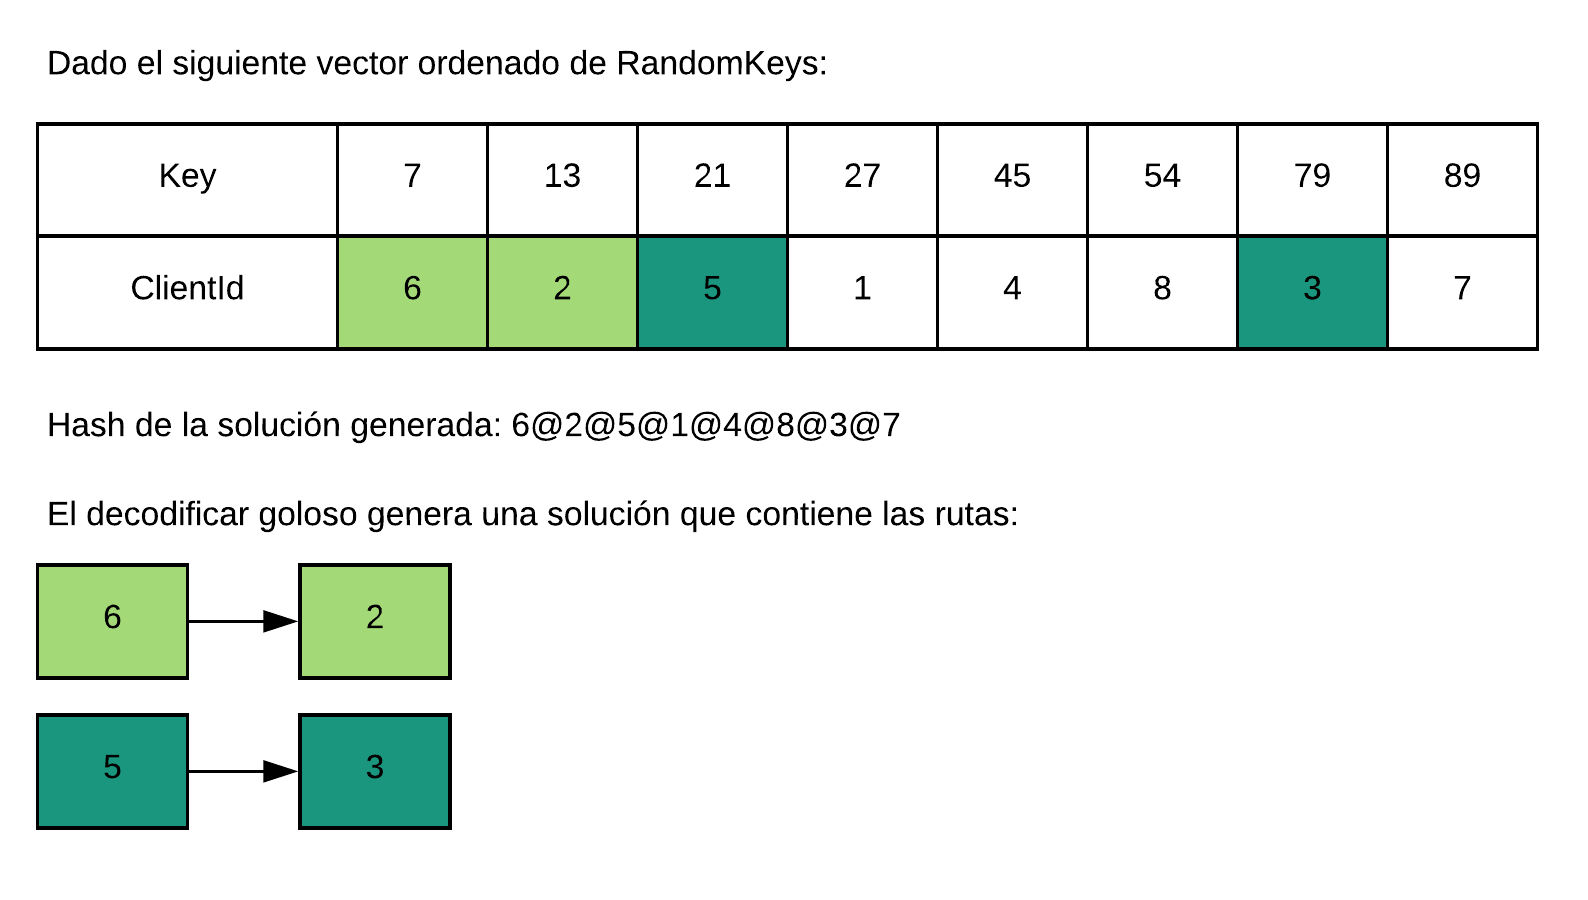
\includegraphics[width=14cm]{codificacionDeSolucionParteUno}
	\label{fig:codificacionDeSolucionUno}
\end{figure}

\begin{figure}[h]
	\caption{Como se actualiza el \textit{RandomKeys} y hash de una solución luego de mejorar la solución \ref{fig:codificacionDeSolucionDos}}
	\centering
	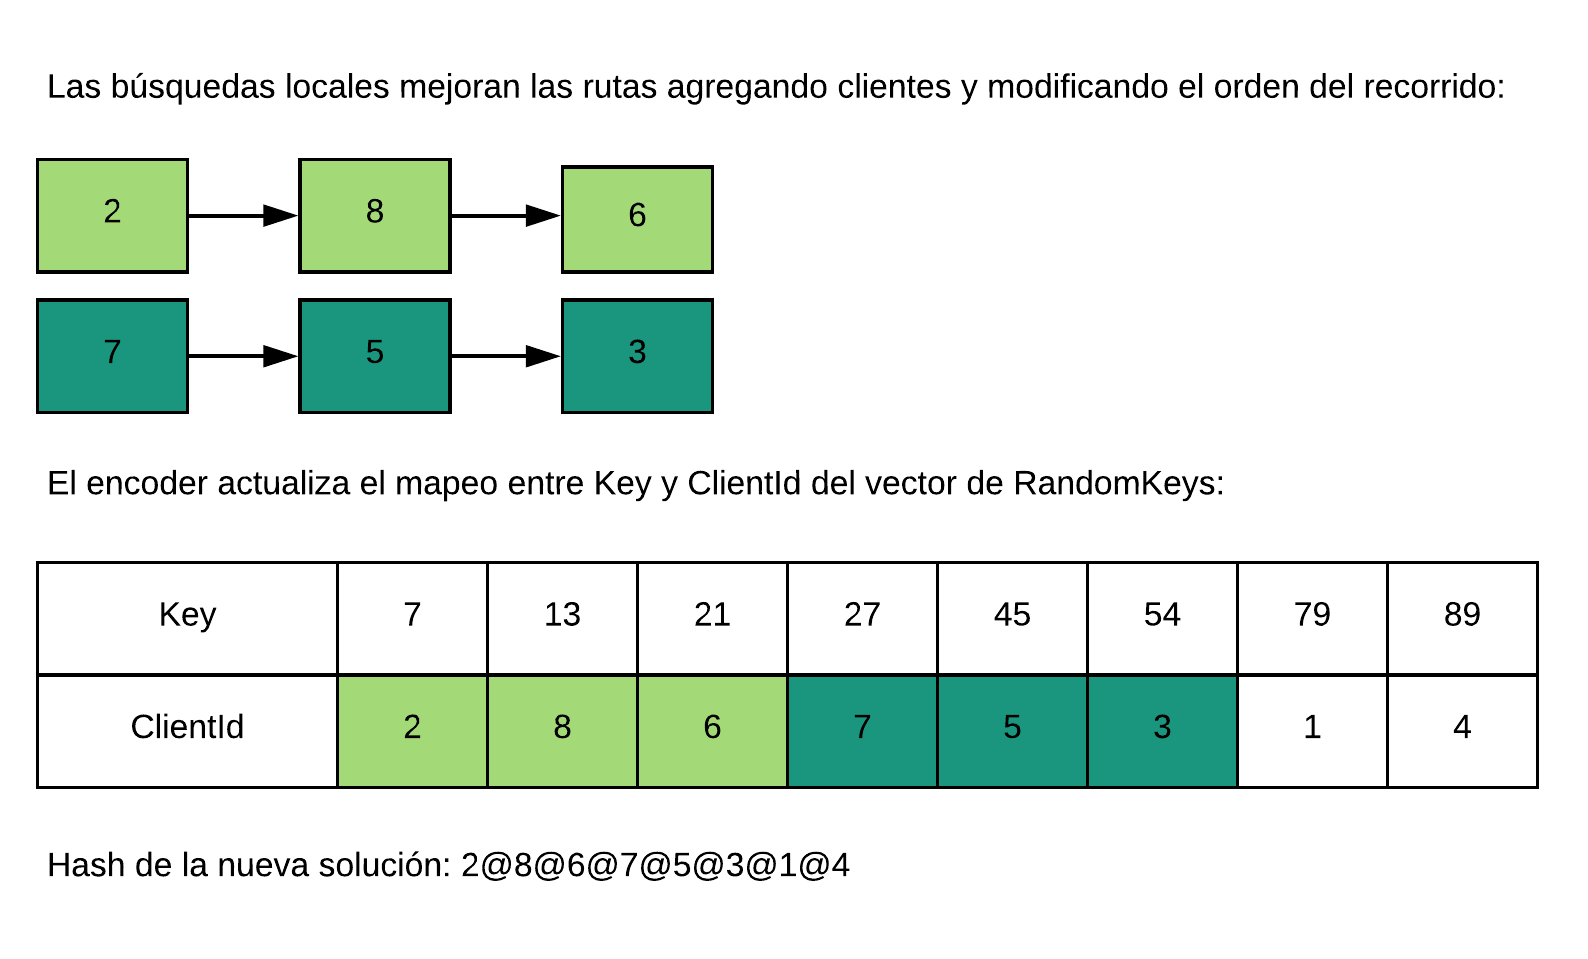
\includegraphics[width=14cm]{codificacionDeSolucionParteDos}
	\label{fig:codificacionDeSolucionDos}
\end{figure}

\bigskip

Ahora bien, digamos que existe un escenario donde el decoder se encuentra trabajando con un RandomKeys que fue generado por el encoder y sucede lo siguiente. Al agregar al último cliente de la primer ruta, como es un decoder goloso, intentará agregar a la primer ruta al resto de los clientes y supongamos que efectivamente encuentra uno. Cuando vi la posibilidad de este escenario, decidi agregar unos delimitadores de modo que si el decoder se encuentra con uno, siempre cambie de vehículo. Estos delimitadores son modelas por la propiedad, \textit{ForceVehicleChangeAfterThis}, con la que extendia al objeto \textit{RandomKey}. De este modo el Decoder, luego de utilizar el \textit{RandomKey}, se fija si \textit{ForceVehicleChangeAfterThis} es \textit{true} y si lo es, deja de intentar agregar clientes a la ruta del vehículo actual, pasando al siguiente. Los delimitadores no son heredados a los descendientes. Estos delimitadores me aseguran que valga: 

\begin{equation} \label{eq:1}
ApplyHeuristic(s) = Decoder.Decode(s.RandomKeys, ProblemInfo)
\end{equation}

\bigskip

En caso de no tener los delimitadores, como dije antes, una ruta podría tener un cliente extra, que para fines del algoritmo, no es malo. Al agregar un cliente, hay dos opciones. La primera es que el cliente perteneciera al subconjunto de clientes que no estaba visitado. En este caso aumentaria el beneficio total. Pero para que esto suceda, la heuristica de insert no debería haber funcionado correctamente ó no fue la última en aplicarse. En caso de que el cliente perteneciece a otro vehículo, el beneficio total no se modifica. El peor escenario es que este segundo vehiculo se quede con el cliente de un tercer vehiculo, sucediendo un especie de cambios en cadenados de clientes entre una secuencia de vehículos sin decrementar el beneficio total. Luego por mas que tomé la desicion de agregar los delimitadores, considero que ambas opciones eran igual de buenas considerando solamente la función objetivo. Como agregar los delimitadores asegura la valides de la ecuación \ref{eq:1}.

%\begin{minipage}{\textwidth}
\begin{lstlisting}
public static Solution UpdateRandomKeys(Solution s);
{
	var randomKeys = s.GetOrderedRandomKeys();
	// Todas las keys ordenadas ascendente
	var keys = randomKeys.Select(k => k.Key).ToList();
	var ClientIds = new List<int>();
	// Get Position Indexes from Visited Clients
	foreach (var r in s.Routes)
	{
		var d = r.GetDestinations();
		var rpi = d.Select(d => d.ClientId);
		ClientIds.AddRange(rpi);
	}
	// Get Position Indexes from Unvisited Clients
	var uClientIds = GetUnvisitedClientIds(randomKeys, newRoutes);
	ClientIdes.AddRange(unvistedClientIdes);

	// Hay un break por cada cantidad de clientes en ruta 
	var breaks = new Queue(newRoutes.Select(r => r.GetDestinations.Count));

	var newRandomKeys = new List<RandomKey>();
	var endRoute = false;
	var acumBreak = 0;
	for (var index = 0; index < keys.Count; index++)
	{
		if (breaks.Count > 0)
		{		
			endRoute = index + 1 == (int)breaks.Peek() + acumBreak;
			if (endRoute)
				acumBreak += (int)breaks.Dequeue();
		}		
		var randomKey = new RandomKey()
		{
			Key = keys[index],
			ClientId = ClientIdes[index],
			ForceVehicleChangeAfterThis = endRoute
		};
		newRandomKeys.Add(randomKey);
	}
	s.SetRandomKeys(newRandomKeys);
	return s;
}
\end{lstlisting}
%\end{minipage}

\subsection{Secuencia de Aplicación de las Heuristicas}

Todas las heuristicas mencionadas, implementan el interfaz:

\begin{lstlisting}
public interface ILocalSearchHeuristic
{
	void ApplyHeuristic(Solution solution);
}
\end{lstlisting}

Esto lo hice así de modo de poder inicializar el vector de heuristicas a aplicar en la creación del algoritmo BRKGA. Luego al momento de aplicar las búsquedas locales, llama en orden de inserción de tal vector y ejecuta su metodo ApplyHeuristic. Así se pueden testear multiples ordenes distintos de búsquedas locales con un simple modificación del parametro de entrada del constructor del BRKGA. El orden en que las heuristicas se aplican es muy relevante. Por ejemplo, si la última heuristica que aplicamos es Swap o 2-Opt, luego la distancias disminuídas de las rutas no sería aprobechado por ninguna cliente.

\bigskip

Configuraciones: 
\begin{itemize}
  \item \textbf{Comun a todas}: MI.200;MNC.50;PS.150;EP.0,3;MP.0,1;EGC.70;TOP.2
  \item \textbf{C = 1}: HEU.IROS;D.G
  \item \textbf{C = 2}: HEU.SIORSOR;D.G
  \item \textbf{C = 3}: HEU.SIORSOR;D.S
  \item \textbf{C = 4}: HEU.SOIR;D.G
  \item \textbf{C = 5}: HEU.SOIR;D.S
  \item \textbf{C = 6}: HEU.SOISOIR;D.G
\end{itemize}

Recordando los codigos de HUE: 
\begin{itemize}
  \item \textbf{I}: Insert (Cliente no visitado)
  \item \textbf{R}: Replace (Cliente no visitado por uno visitado)
  \item \textbf{0}: 2-Opt (Swap dentro de una misma ruta)
  \item \textbf{S}: Swap (Swap entre dos rutas distintas)
\end{itemize}

\bigskip

Genere soluciones para las mismas seis instancias diversas, varian en la configuración solamente el orden de las búsquedas locales y el decodificador obteniendo los siguientes resultados:

\bigskip

\begin{center}
\begin{tabular}{ |c|c|c|c|c|c|c|c|c|c|c|c| } 
\hline
$I$ & $\#N$ & $\#V$ & $tMax$ & $C$ & $\#S$ & $t_{avg}$ & $B_{max}$ & $B_{min}$ & $B_{avg}$ & $i_{f}$ & $BTP_{max}$ \\
\hline
p2.2.k & 21 & 2 & 22.50 & 1 & 10 & 4724 & 275 & 260 & 267 & 0.97 & 275  \\
p2.2.k & 21 & 2 & 22.50 & 2 & 10 & 5136 & 275 & 260 & 268 & 0.97 & 275  \\
p2.2.k & 21 & 2 & 22.50 & 3 & 10 & 3333 & 275 & 260 & 268 & 0.97 & 275  \\
p2.2.k & 21 & 2 & 22.50 & 4 & 10 & 4410 & 270 & 260 & 269 & 0.98 & 275  \\
p2.2.k & 21 & 2 & 22.50 & 5 & 10 & 2610 & 270 & 260 & 267 & 0.97 & 275  \\
p2.2.k & 21 & 2 & 22.50 & 6 & 10 & 4884 & 270 & 265 & 269 & 0.98 & 275  \\
p2.3.g & 21 & 3 & 10.70 & 1 & 10 & 2710 & 145 & 145 & 145 & 1.00 & 145  \\
p2.3.g & 21 & 3 & 10.70 & 2 & 10 & 3025 & 145 & 145 & 145 & 1.00 & 145  \\
p2.3.g & 21 & 3 & 10.70 & 3 & 10 & 2047 & 145 & 145 & 145 & 1.00 & 145  \\
p2.3.g & 21 & 3 & 10.70 & 4 & 10 & 2880 & 145 & 145 & 145 & 1.00 & 145  \\
p2.3.g & 21 & 3 & 10.70 & 5 & 10 & 1954 & 145 & 145 & 145 & 1.00 & 145  \\
p2.3.g & 21 & 3 & 10.70 & 6 & 10 & 2883 & 145 & 145 & 145 & 1.00 & 145  \\
p3.4.p & 33 & 4 & 22.50 & 1 & 10 & 10613 & 540 & 510 & 524 & 0.94 & 560  \\
p3.4.p & 33 & 4 & 22.50 & 2 & 10 & 11692 & 540 & 540 & 540 & 0.96 & 560  \\
p3.4.p & 33 & 4 & 22.50 & 3 & 10 & 5361 & 560 & 540 & 550 & 0.98 & 560  \\
p3.4.p & 33 & 4 & 22.50 & 4 & 10 & 10341 & 540 & 540 & 540 & 0.96 & 560  \\
p3.4.p & 33 & 4 & 22.50 & 5 & 10 & 4101 & 560 & 540 & 550 & 0.98 & 560  \\
p3.4.p & 33 & 4 & 22.50 & 6 & 10 & 11247 & 560 & 540 & 543 & 0.97 & 560  \\
p5.3.x & 66 & 3 & 40.00 & 1 & 10 & 32077 & 1435 & 1340 & 1382 & 0.89 & 1555  \\
p5.3.x & 66 & 3 & 40.00 & 2 & 10 & 39871 & 1505 & 1475 & 1489 & 0.96 & 1555  \\
p5.3.x & 66 & 3 & 40.00 & 3 & 10 & 19296 & 1505 & 1470 & 1487 & 0.96 & 1555  \\
p5.3.x & 66 & 3 & 40.00 & 4 & 10 & 32672 & 1485 & 1450 & 1464 & 0.94 & 1555  \\
p5.3.x & 66 & 3 & 40.00 & 5 & 10 & 10854 & 1490 & 1425 & 1454 & 0.94 & 1555  \\
p5.3.x & 66 & 3 & 40.00 & 6 & 10 & 35290 & 1490 & 1455 & 1469 & 0.94 & 1555  \\
p7.2.e & 102 & 2 & 50.00 & 1 & 10 & 14956 & 290 & 280 & 286 & 0.99 & 290  \\
p7.2.e & 102 & 2 & 50.00 & 2 & 10 & 15837 & 290 & 285 & 289 & 1.00 & 290  \\
p7.2.e & 102 & 2 & 50.00 & 3 & 10 & 8859 & 290 & 289 & 289 & 1.00 & 290  \\
p7.2.e & 102 & 2 & 50.00 & 4 & 10 & 13623 & 290 & 290 & 290 & 1.00 & 290  \\
p7.2.e & 102 & 2 & 50.00 & 5 & 10 & 6605 & 290 & 285 & 289 & 1.00 & 290  \\
p7.2.e & 102 & 2 & 50.00 & 6 & 10 & 14637 & 290 & 281 & 288 & 0.99 & 290  \\
p7.4.t & 102 & 4 & 100.00 & 1 & 10 & 57849 & 988 & 925 & 949 & 0.88 & 1077  \\
p7.4.t & 102 & 4 & 100.00 & 2 & 10 & 66773 & 1008 & 978 & 995 & 0.92 & 1077  \\
p7.4.t & 102 & 4 & 100.00 & 3 & 10 & 33420 & 1020 & 979 & 997 & 0.93 & 1077  \\
p7.4.t & 102 & 4 & 100.00 & 4 & 10 & 52095 & 1003 & 957 & 983 & 0.91 & 1077  \\
p7.4.t & 102 & 4 & 100.00 & 5 & 10 & 18879 & 1015 & 963 & 989 & 0.92 & 1077  \\
p7.4.t & 102 & 4 & 100.00 & 6 & 10 & 57895 & 1012 & 955 & 983 & 0.91 & 1077  \\
\hline
\end{tabular}
\end{center}

\bigskip

Observaciones de estos resultados:

\bigskip

Claramente el peor orden de heuristicas locales es IROS (Insert, Replace, 2-Opt, Swap). Esto es por lo que explicamos anteriormente, Insert y Replace intentan agregar mas clientes o intercambiar clientes mas rentables mejorando el beneficio de la ruta. Mientras que 2-Opt y Swap hacen un reordenamiento de la secuencia en que se visitan los clientes seleccionados, luego minimizan la distancia recorrida de una ruta. Al primero los de beneficio y luego los de distancia, no se utiliza la distancia ahorrada.

\bigskip

Luego el mejor orden segun estos resultados, fue SIORSOR. Notar que repito heuristicas en este orden, esto en una primera impresión parece redundante pero no lo es. Por ejemplo, la primera vez que se aplica 2-opt se hace luego de un Insert que utiliza toda la distancia disponible. Y la segunda vez que se aplica el 2-opt es luego de un Swap que modifico rutas de forma tal que quiza disminuyo la distancia recorrida.

\bigskip

Sobre $T_{avg}$, notar entre la configuración 2 y 3 el tiempo puede llegar a ser más del doble y la única diferencia es que se uso el decodificador simple vs el goloso. Esto lo logra con un $i_f$ prácticamente igual en todas las intancias. Lo mismo podemos observar entre la configuración 4 y 5. Por lo tanto, habiendo agregado las heuristicas de búsqueda local, el decodificador goloso no mejora el beneficio final y el decodificador simple reduce el tiempo de ejecución. Por este motivo para los resultados finales utilicé el decodificar simple.


